\textbf{\underline{OZ 3 - De Lorentzkracht en de wet van Ampère - Oefening 4:}}
\vspace{0.5cm}

% \begin{description}[labelwidth=1.5cm, leftmargin=!]
%     \item[Geg. :]   
%     \item[Gevr. :]  
%     \item[Opl. :]  
% \end{description}

\begin{minipage}{.76\textwidth}
    Hiernaast is een coaxiale kabel afgebeeld. Rond de binnenste geleider zit een isolerender laag, daarbuiten zit opnieuw een geleidende laag die afgeschermd wordt met een tweede laag isolatiemateriaal. De stroom door de binnenste draad is $1.00$ A \textbf{uit} het blad, de stroom door de buitenste geleider is $3.00$ A \textbf{in} het blad. Wat is de grootte, richting en zin van het magnetische veld in punten $a$ en $b$?

    \vspace{1cm}
\end{minipage}
\begin{minipage}{.2\textwidth}
    \vspace{-0.5cm}
    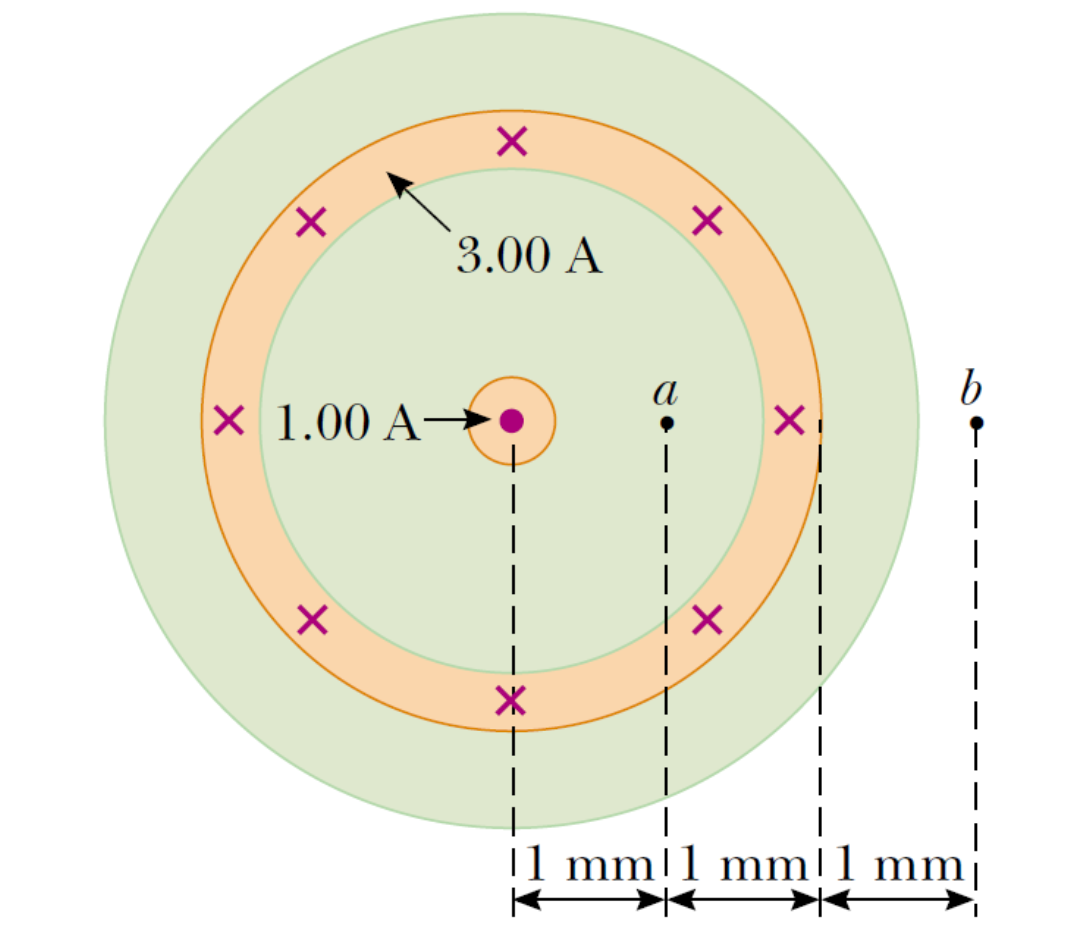
\includegraphics[scale = 0.225]{oz03/resources/Oz3Oef4.png}
\end{minipage}

\vspace{-0.9cm}

\begin{description}[labelwidth=1.5cm, leftmargin=!]
    \item[Geg. :]   $I_{\text{binnen}} = 1.00$ A, $I_{\text{buiten}} = 3.00$ A, $r_a = 1 \cdot 10^{-3}$ m, $r_b = 3r_a = 3 \cdot 10^{-3}$ m
    \item[Gevr. :]  $\Vec{B}_a$, $\Vec{B}_b$ ?
    \item[Opl. :]   
                    \begin{enumerate}[(a)]
                        \item
                            We passen de wet van ampère toe op het punt:
                            \begin{equation*}
                                B_a = \dfrac{\mu_0I_{\text{binnen}}}{2\pi r_a} = 2.00 \cdot 10^{-4} \text{ T}
                            \end{equation*}
                            Vectorieel wordt dit:
                            \begin{equation*}
                                \Vec{B}_a = 2.00 \cdot 10^{-4} \text{ T } \hat{j}
                            \end{equation*}
                            % sinds de ingesloten stroom uit het blad is.
                        \item 
                            We passen de wet van ampère toe op het punt:
                            \begin{equation*}
                                B_b = \dfrac{\mu_0}{2\pi r_a}(I_{\text{binnen}} + I_{\text{buiten}}) = -1.33 \cdot 10^{-4} \text{ T}
                            \end{equation*}
                            Vectorieel wordt dit:
                            \begin{equation*}
                                \Vec{B}_b = 1.33 \cdot 10^{-4} \text{ T }  (-\hat{j})
                            \end{equation*}
                            % sinds de ingesloten stroom in het blad is.
                    \end{enumerate}

                    
\end{description}

\vspace{1cm}
